\documentclass[1p]{elsarticle_modified}
%\bibliographystyle{elsarticle-num}

%\usepackage[colorlinks]{hyperref}
%\usepackage{abbrmath_seonhwa} %\Abb, \Ascr, \Acal ,\Abf, \Afrak
\usepackage{amsfonts}
\usepackage{amssymb}
\usepackage{amsmath}
\usepackage{amsthm}
\usepackage{scalefnt}
\usepackage{amsbsy}
\usepackage{kotex}
\usepackage{caption}
\usepackage{subfig}
\usepackage{color}
\usepackage{graphicx}
\usepackage{xcolor} %% white, black, red, green, blue, cyan, magenta, yellow
\usepackage{float}
\usepackage{setspace}
\usepackage{hyperref}

\usepackage{tikz}
\usetikzlibrary{arrows}

\usepackage{multirow}
\usepackage{array} % fixed length table
\usepackage{hhline}

%%%%%%%%%%%%%%%%%%%%%
\makeatletter
\renewcommand*\env@matrix[1][\arraystretch]{%
	\edef\arraystretch{#1}%
	\hskip -\arraycolsep
	\let\@ifnextchar\new@ifnextchar
	\array{*\c@MaxMatrixCols c}}
\makeatother %https://tex.stackexchange.com/questions/14071/how-can-i-increase-the-line-spacing-in-a-matrix
%%%%%%%%%%%%%%%

\usepackage[normalem]{ulem}

\newcommand{\msout}[1]{\ifmmode\text{\sout{\ensuremath{#1}}}\else\sout{#1}\fi}
%SOURCE: \msout is \stkout macro in https://tex.stackexchange.com/questions/20609/strikeout-in-math-mode

\newcommand{\cancel}[1]{
	\ifmmode
	{\color{red}\msout{#1}}
	\else
	{\color{red}\sout{#1}}
	\fi
}

\newcommand{\add}[1]{
	{\color{blue}\uwave{#1}}
}

\newcommand{\replace}[2]{
	\ifmmode
	{\color{red}\msout{#1}}{\color{blue}\uwave{#2}}
	\else
	{\color{red}\sout{#1}}{\color{blue}\uwave{#2}}
	\fi
}

\newcommand{\Sol}{\mathcal{S}} %segment
\newcommand{\D}{D} %diagram
\newcommand{\A}{\mathcal{A}} %arc


%%%%%%%%%%%%%%%%%%%%%%%%%%%%%5 test

\def\sl{\operatorname{\textup{SL}}(2,\Cbb)}
\def\psl{\operatorname{\textup{PSL}}(2,\Cbb)}
\def\quan{\mkern 1mu \triangleright \mkern 1mu}

\theoremstyle{definition}
\newtheorem{thm}{Theorem}[section]
\newtheorem{prop}[thm]{Proposition}
\newtheorem{lem}[thm]{Lemma}
\newtheorem{ques}[thm]{Question}
\newtheorem{cor}[thm]{Corollary}
\newtheorem{defn}[thm]{Definition}
\newtheorem{exam}[thm]{Example}
\newtheorem{rmk}[thm]{Remark}
\newtheorem{alg}[thm]{Algorithm}

\newcommand{\I}{\sqrt{-1}}
\begin{document}

%\begin{frontmatter}
%
%\title{Boundary parabolic representations of knots up to 8 crossings}
%
%%% Group authors per affiliation:
%\author{Yunhi Cho} 
%\address{Department of Mathematics, University of Seoul, Seoul, Korea}
%\ead{yhcho@uos.ac.kr}
%
%
%\author{Seonhwa Kim} %\fnref{s_kim}}
%\address{Center for Geometry and Physics, Institute for Basic Science, Pohang, 37673, Korea}
%\ead{ryeona17@ibs.re.kr}
%
%\author{Hyuk Kim}
%\address{Department of Mathematical Sciences, Seoul National University, Seoul 08826, Korea}
%\ead{hyukkim@snu.ac.kr}
%
%\author{Seokbeom Yoon}
%\address{Department of Mathematical Sciences, Seoul National University, Seoul, 08826,  Korea}
%\ead{sbyoon15@snu.ac.kr}
%
%\begin{abstract}
%We find all boundary parabolic representation of knots up to 8 crossings.
%
%\end{abstract}
%\begin{keyword}
%    \MSC[2010] 57M25 
%\end{keyword}
%
%\end{frontmatter}

%\linenumbers
%\tableofcontents
%
\newcommand\colored[1]{\textcolor{white}{\rule[-0.35ex]{0.8em}{1.4ex}}\kern-0.8em\color{red} #1}%
%\newcommand\colored[1]{\textcolor{white}{ #1}\kern-2.17ex	\textcolor{white}{ #1}\kern-1.81ex	\textcolor{white}{ #1}\kern-2.15ex\color{red}#1	}

{\Large $\underline{11n_{7}~(K11n_{7})}$}

\setlength{\tabcolsep}{10pt}
\renewcommand{\arraystretch}{1.6}
\vspace{1cm}\begin{tabular}{m{100pt}>{\centering\arraybackslash}m{274pt}}
\multirow{5}{120pt}{
	\centering
	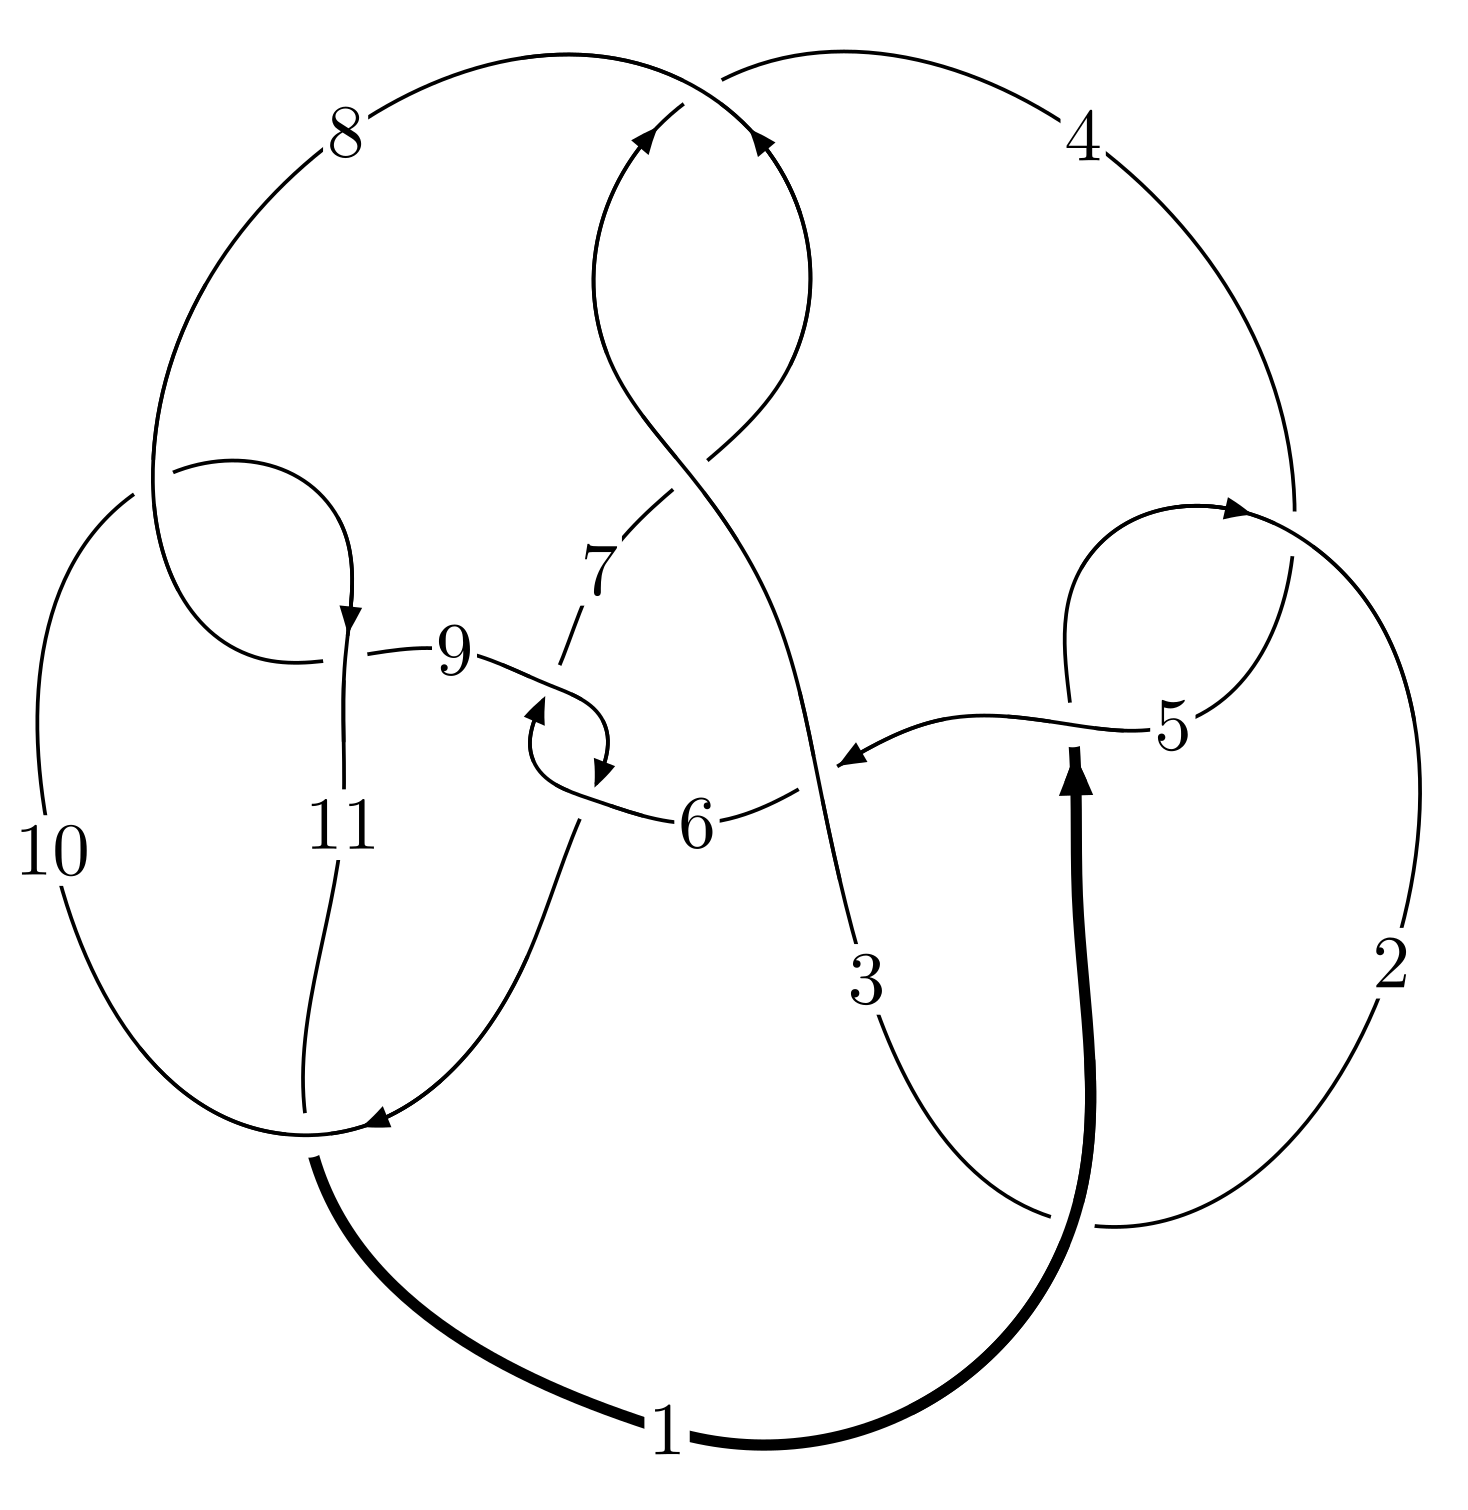
\includegraphics[width=112pt]{../../../GIT/diagram.site/Diagrams/png/623_11n_7.png}\\
\ \ \ A knot diagram\footnotemark}&
\allowdisplaybreaks
\textbf{Linearized knot diagam} \\
\cline{2-2}
 &
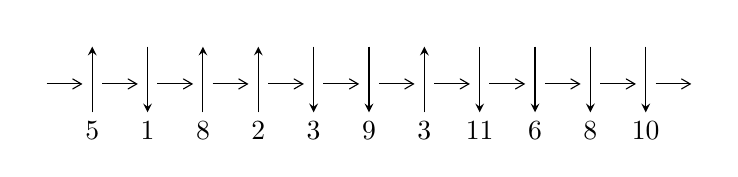
\begin{tikzpicture}[x=20pt, y=17pt]
	% nodes
	\node (C0) at (0, 0) {};
	\node (C1) at (1, 0) {};
	\node (C1U) at (1, +1) {};
	\node (C1D) at (1, -1) {5};

	\node (C2) at (2, 0) {};
	\node (C2U) at (2, +1) {};
	\node (C2D) at (2, -1) {1};

	\node (C3) at (3, 0) {};
	\node (C3U) at (3, +1) {};
	\node (C3D) at (3, -1) {8};

	\node (C4) at (4, 0) {};
	\node (C4U) at (4, +1) {};
	\node (C4D) at (4, -1) {2};

	\node (C5) at (5, 0) {};
	\node (C5U) at (5, +1) {};
	\node (C5D) at (5, -1) {3};

	\node (C6) at (6, 0) {};
	\node (C6U) at (6, +1) {};
	\node (C6D) at (6, -1) {9};

	\node (C7) at (7, 0) {};
	\node (C7U) at (7, +1) {};
	\node (C7D) at (7, -1) {3};

	\node (C8) at (8, 0) {};
	\node (C8U) at (8, +1) {};
	\node (C8D) at (8, -1) {11};

	\node (C9) at (9, 0) {};
	\node (C9U) at (9, +1) {};
	\node (C9D) at (9, -1) {6};

	\node (C10) at (10, 0) {};
	\node (C10U) at (10, +1) {};
	\node (C10D) at (10, -1) {8};

	\node (C11) at (11, 0) {};
	\node (C11U) at (11, +1) {};
	\node (C11D) at (11, -1) {10};
	\node (C12) at (12, 0) {};

	% arrows
	\draw[->,>={angle 60}]
	(C0) edge (C1) (C1) edge (C2) (C2) edge (C3) (C3) edge (C4) (C4) edge (C5) (C5) edge (C6) (C6) edge (C7) (C7) edge (C8) (C8) edge (C9) (C9) edge (C10) (C10) edge (C11) (C11) edge (C12) ;	\draw[->,>=stealth]
	(C1D) edge (C1U) (C2U) edge (C2D) (C3D) edge (C3U) (C4D) edge (C4U) (C5U) edge (C5D) (C6U) edge (C6D) (C7D) edge (C7U) (C8U) edge (C8D) (C9U) edge (C9D) (C10U) edge (C10D) (C11U) edge (C11D) ;
	\end{tikzpicture} \\
\hhline{~~} \\& 
\textbf{Solving Sequence} \\ \cline{2-2} 
 &
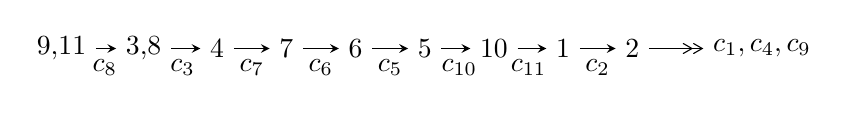
\begin{tikzpicture}[x=25pt, y=7pt]
	% node
	\node (A0) at (-1/8, 0) {9,11};
	\node (A1) at (17/16, 0) {3,8};
	\node (A2) at (17/8, 0) {4};
	\node (A3) at (25/8, 0) {7};
	\node (A4) at (33/8, 0) {6};
	\node (A5) at (41/8, 0) {5};
	\node (A6) at (49/8, 0) {10};
	\node (A7) at (57/8, 0) {1};
	\node (A8) at (65/8, 0) {2};
	\node (C1) at (1/2, -1) {$c_{8}$};
	\node (C2) at (13/8, -1) {$c_{3}$};
	\node (C3) at (21/8, -1) {$c_{7}$};
	\node (C4) at (29/8, -1) {$c_{6}$};
	\node (C5) at (37/8, -1) {$c_{5}$};
	\node (C6) at (45/8, -1) {$c_{10}$};
	\node (C7) at (53/8, -1) {$c_{11}$};
	\node (C8) at (61/8, -1) {$c_{2}$};
	\node (A9) at (10, 0) {$c_{1},c_{4},c_{9}$};

	% edge
	\draw[->,>=stealth]	
	(A0) edge (A1) (A1) edge (A2) (A2) edge (A3) (A3) edge (A4) (A4) edge (A5) (A5) edge (A6) (A6) edge (A7) (A7) edge (A8) ;
	\draw[->>,>={angle 60}]	
	(A8) edge (A9);
\end{tikzpicture} \\ 

\end{tabular} \\

\footnotetext{
The image of knot diagram is generated by the software ``\textbf{Draw programme}" developed by Andrew Bartholomew(\url{http://www.layer8.co.uk/maths/draw/index.htm\#Running-draw}), where we modified some parts for our purpose(\url{https://github.com/CATsTAILs/LinksPainter}).
}\phantom \\ \newline 
\centering \textbf{Ideals for irreducible components\footnotemark of $X_{\text{par}}$} 
 
\begin{align*}
I^u_{1}&=\langle 
2.20194\times10^{21} u^{38}+4.46582\times10^{22} u^{37}+\cdots+2.15629\times10^{22} b+5.77763\times10^{22},\\
\phantom{I^u_{1}}&\phantom{= \langle  }-5.60651\times10^{22} u^{38}-2.01892\times10^{23} u^{37}+\cdots+2.15629\times10^{22} a+8.89136\times10^{22},\;u^{39}+3 u^{38}+\cdots-5 u-1\rangle \\
I^u_{2}&=\langle 
u^2 a+b,\;u^2 a+a^2+2 a u+3 u^2+a+5 u+4,\;u^3+u^2-1\rangle \\
\\
\end{align*}
\raggedright * 2 irreducible components of $\dim_{\mathbb{C}}=0$, with total 45 representations.\\
\footnotetext{All coefficients of polynomials are rational numbers. But the coefficients are sometimes approximated in decimal forms when there is not enough margin.}
\newpage
\renewcommand{\arraystretch}{1}
\centering \section*{I. $I^u_{1}= \langle 2.20\times10^{21} u^{38}+4.47\times10^{22} u^{37}+\cdots+2.16\times10^{22} b+5.78\times10^{22},\;-5.61\times10^{22} u^{38}-2.02\times10^{23} u^{37}+\cdots+2.16\times10^{22} a+8.89\times10^{22},\;u^{39}+3 u^{38}+\cdots-5 u-1 \rangle$}
\flushleft \textbf{(i) Arc colorings}\\
\begin{tabular}{m{7pt} m{180pt} m{7pt} m{180pt} }
\flushright $a_{9}=$&$\begin{pmatrix}1\\0\end{pmatrix}$ \\
\flushright $a_{11}=$&$\begin{pmatrix}0\\u\end{pmatrix}$ \\
\flushright $a_{3}=$&$\begin{pmatrix}2.60007 u^{38}+9.36292 u^{37}+\cdots-11.3955 u-4.12344\\-0.102117 u^{38}-2.07106 u^{37}+\cdots-13.0171 u-2.67943\end{pmatrix}$ \\
\flushright $a_{8}=$&$\begin{pmatrix}1\\- u^2\end{pmatrix}$ \\
\flushright $a_{4}=$&$\begin{pmatrix}2.79441 u^{38}+10.0298 u^{37}+\cdots-13.9989 u-5.24015\\-0.0584579 u^{38}-2.06978 u^{37}+\cdots-13.6305 u-2.76324\end{pmatrix}$ \\
\flushright $a_{7}=$&$\begin{pmatrix}-0.700760 u^{38}-0.594268 u^{37}+\cdots+7.97882 u-0.0611499\\-1.25362 u^{38}-2.81386 u^{37}+\cdots+0.0129788 u-0.500639\end{pmatrix}$ \\
\flushright $a_{6}=$&$\begin{pmatrix}-1.95438 u^{38}-3.40813 u^{37}+\cdots+7.99180 u-0.561789\\-1.25362 u^{38}-2.81386 u^{37}+\cdots+0.0129788 u-0.500639\end{pmatrix}$ \\
\flushright $a_{5}=$&$\begin{pmatrix}2.47112 u^{38}+9.86388 u^{37}+\cdots+8.27156 u+1.66377\\-0.721787 u^{38}-4.52792 u^{37}+\cdots-15.7237 u-2.45051\end{pmatrix}$ \\
\flushright $a_{10}=$&$\begin{pmatrix}u\\- u^3+u\end{pmatrix}$ \\
\flushright $a_{1}=$&$\begin{pmatrix}- u^3\\u^5- u^3+u\end{pmatrix}$ \\
\flushright $a_{2}=$&$\begin{pmatrix}2.46841 u^{38}+9.39037 u^{37}+\cdots-9.44573 u-3.72104\\-0.0315650 u^{38}-2.27311 u^{37}+\cdots-14.5271 u-2.54332\end{pmatrix}$\\ \flushright $a_{2}=$&$\begin{pmatrix}2.46841 u^{38}+9.39037 u^{37}+\cdots-9.44573 u-3.72104\\-0.0315650 u^{38}-2.27311 u^{37}+\cdots-14.5271 u-2.54332\end{pmatrix}$\\&\end{tabular}
\flushleft \textbf{(ii) Obstruction class $= -1$}\\~\\
\flushleft \textbf{(iii) Cusp Shapes $= \frac{95167190231219974262615}{10781474718762665439818} u^{38}+\frac{642665286688782560331753}{21562949437525330879636} u^{37}+\cdots+\frac{910083121628952116105487}{10781474718762665439818} u+\frac{469851565658388329096693}{21562949437525330879636}$}\\~\\
\newpage\renewcommand{\arraystretch}{1}
\flushleft \textbf{(iv) u-Polynomials at the component}\newline \\
\begin{tabular}{m{50pt}|m{274pt}}
Crossings & \hspace{64pt}u-Polynomials at each crossing \\
\hline $$\begin{aligned}c_{1},c_{4}\end{aligned}$$&$\begin{aligned}
&u^{39}+4 u^{38}+\cdots+10 u-1
\end{aligned}$\\
\hline $$\begin{aligned}c_{2}\end{aligned}$$&$\begin{aligned}
&u^{39}+22 u^{38}+\cdots+170 u-1
\end{aligned}$\\
\hline $$\begin{aligned}c_{3},c_{7}\end{aligned}$$&$\begin{aligned}
&u^{39}+3 u^{38}+\cdots+160 u+64
\end{aligned}$\\
\hline $$\begin{aligned}c_{5}\end{aligned}$$&$\begin{aligned}
&u^{39}-4 u^{38}+\cdots+602 u-49
\end{aligned}$\\
\hline $$\begin{aligned}c_{6},c_{9}\end{aligned}$$&$\begin{aligned}
&u^{39}-3 u^{38}+\cdots-3 u+1
\end{aligned}$\\
\hline $$\begin{aligned}c_{8},c_{10}\end{aligned}$$&$\begin{aligned}
&u^{39}-3 u^{38}+\cdots-5 u+1
\end{aligned}$\\
\hline $$\begin{aligned}c_{11}\end{aligned}$$&$\begin{aligned}
&u^{39}+23 u^{38}+\cdots+u+1
\end{aligned}$\\
\hline
\end{tabular}\\~\\
\newpage\renewcommand{\arraystretch}{1}
\flushleft \textbf{(v) Riley Polynomials at the component}\newline \\
\begin{tabular}{m{50pt}|m{274pt}}
Crossings & \hspace{64pt}Riley Polynomials at each crossing \\
\hline $$\begin{aligned}c_{1},c_{4}\end{aligned}$$&$\begin{aligned}
&y^{39}+22 y^{38}+\cdots+170 y-1
\end{aligned}$\\
\hline $$\begin{aligned}c_{2}\end{aligned}$$&$\begin{aligned}
&y^{39}-6 y^{38}+\cdots+31510 y-1
\end{aligned}$\\
\hline $$\begin{aligned}c_{3},c_{7}\end{aligned}$$&$\begin{aligned}
&y^{39}+35 y^{38}+\cdots-23552 y-4096
\end{aligned}$\\
\hline $$\begin{aligned}c_{5}\end{aligned}$$&$\begin{aligned}
&y^{39}-34 y^{38}+\cdots+391706 y-2401
\end{aligned}$\\
\hline $$\begin{aligned}c_{6},c_{9}\end{aligned}$$&$\begin{aligned}
&y^{39}+9 y^{38}+\cdots+y-1
\end{aligned}$\\
\hline $$\begin{aligned}c_{8},c_{10}\end{aligned}$$&$\begin{aligned}
&y^{39}-23 y^{38}+\cdots+y-1
\end{aligned}$\\
\hline $$\begin{aligned}c_{11}\end{aligned}$$&$\begin{aligned}
&y^{39}-11 y^{38}+\cdots+117 y-1
\end{aligned}$\\
\hline
\end{tabular}\\~\\
\newpage\flushleft \textbf{(vi) Complex Volumes and Cusp Shapes}
$$\begin{array}{c|c|c}  
\text{Solutions to }I^u_{1}& \I (\text{vol} + \sqrt{-1}CS) & \text{Cusp shape}\\
 \hline 
\begin{aligned}
u &= \phantom{-}0.174715 + 0.953666 I \\
a &= -0.107736 - 0.141147 I \\
b &= -0.224524 + 1.376020 I\end{aligned}
 & -5.68977 + 0.80789 I & -5.63151 - 0.39749 I \\ \hline\begin{aligned}
u &= \phantom{-}0.174715 - 0.953666 I \\
a &= -0.107736 + 0.141147 I \\
b &= -0.224524 - 1.376020 I\end{aligned}
 & -5.68977 - 0.80789 I & -5.63151 + 0.39749 I \\ \hline\begin{aligned}
u &= -0.113785 + 1.039480 I \\
a &= \phantom{-}0.1112140 + 0.0706545 I \\
b &= -0.41499 + 1.53589 I\end{aligned}
 & -4.49350 - 8.17612 I & -3.77298 + 5.44747 I \\ \hline\begin{aligned}
u &= -0.113785 - 1.039480 I \\
a &= \phantom{-}0.1112140 - 0.0706545 I \\
b &= -0.41499 - 1.53589 I\end{aligned}
 & -4.49350 + 8.17612 I & -3.77298 - 5.44747 I \\ \hline\begin{aligned}
u &= -0.906304 + 0.258793 I \\
a &= -0.59831 + 2.09555 I \\
b &= -0.938219 - 0.467153 I\end{aligned}
 & \phantom{-}0.05191 + 4.16636 I & -0.57665 - 9.00427 I \\ \hline\begin{aligned}
u &= -0.906304 - 0.258793 I \\
a &= -0.59831 - 2.09555 I \\
b &= -0.938219 + 0.467153 I\end{aligned}
 & \phantom{-}0.05191 - 4.16636 I & -0.57665 + 9.00427 I \\ \hline\begin{aligned}
u &= \phantom{-}0.913889 + 0.058300 I \\
a &= \phantom{-}0.77201 + 4.31604 I \\
b &= -0.20598 - 3.29592 I\end{aligned}
 & -1.32570 - 2.15384 I & -38.3073 + 0.3658 I \\ \hline\begin{aligned}
u &= \phantom{-}0.913889 - 0.058300 I \\
a &= \phantom{-}0.77201 - 4.31604 I \\
b &= -0.20598 + 3.29592 I\end{aligned}
 & -1.32570 + 2.15384 I & -38.3073 - 0.3658 I \\ \hline\begin{aligned}
u &= \phantom{-}0.814464 + 0.380892 I \\
a &= \phantom{-}0.328778 + 0.693706 I \\
b &= -0.352686 - 1.052600 I\end{aligned}
 & -1.92828 + 0.12066 I & -7.15424 - 0.12690 I \\ \hline\begin{aligned}
u &= \phantom{-}0.814464 - 0.380892 I \\
a &= \phantom{-}0.328778 - 0.693706 I \\
b &= -0.352686 + 1.052600 I\end{aligned}
 & -1.92828 - 0.12066 I & -7.15424 + 0.12690 I\\
 \hline 
 \end{array}$$\newpage$$\begin{array}{c|c|c}  
\text{Solutions to }I^u_{1}& \I (\text{vol} + \sqrt{-1}CS) & \text{Cusp shape}\\
 \hline 
\begin{aligned}
u &= -0.062003 + 0.891851 I \\
a &= \phantom{-}0.073492 - 0.130422 I \\
b &= \phantom{-}0.43523 - 1.38427 I\end{aligned}
 & -1.45248 - 3.13609 I & -0.74981 + 2.49452 I \\ \hline\begin{aligned}
u &= -0.062003 - 0.891851 I \\
a &= \phantom{-}0.073492 + 0.130422 I \\
b &= \phantom{-}0.43523 + 1.38427 I\end{aligned}
 & -1.45248 + 3.13609 I & -0.74981 - 2.49452 I \\ \hline\begin{aligned}
u &= -0.791534 + 0.793494 I \\
a &= -0.286108 + 0.284239 I \\
b &= \phantom{-}0.033088 + 0.170270 I\end{aligned}
 & \phantom{-}2.88333 + 1.52566 I & -2.95623 - 6.42875 I \\ \hline\begin{aligned}
u &= -0.791534 - 0.793494 I \\
a &= -0.286108 - 0.284239 I \\
b &= \phantom{-}0.033088 - 0.170270 I\end{aligned}
 & \phantom{-}2.88333 - 1.52566 I & -2.95623 + 6.42875 I \\ \hline\begin{aligned}
u &= -1.105650 + 0.283891 I \\
a &= -0.916031 - 0.529536 I \\
b &= -0.320477 + 0.011103 I\end{aligned}
 & -3.35360 + 5.46941 I & -6.70822 - 8.69559 I \\ \hline\begin{aligned}
u &= -1.105650 - 0.283891 I \\
a &= -0.916031 + 0.529536 I \\
b &= -0.320477 - 0.011103 I\end{aligned}
 & -3.35360 - 5.46941 I & -6.70822 + 8.69559 I \\ \hline\begin{aligned}
u &= \phantom{-}1.155090 + 0.139104 I \\
a &= -0.289265 - 1.321470 I \\
b &= \phantom{-}0.71983 + 1.54185 I\end{aligned}
 & -2.82585 - 1.96097 I & -4.21009 + 0.40138 I \\ \hline\begin{aligned}
u &= \phantom{-}1.155090 - 0.139104 I \\
a &= -0.289265 + 1.321470 I \\
b &= \phantom{-}0.71983 - 1.54185 I\end{aligned}
 & -2.82585 + 1.96097 I & -4.21009 - 0.40138 I \\ \hline\begin{aligned}
u &= \phantom{-}0.833700\phantom{ +0.000000I} \\
a &= \phantom{-}0.604067\phantom{ +0.000000I} \\
b &= -0.694607\phantom{ +0.000000I}\end{aligned}
 & -1.20362\phantom{ +0.000000I} & -8.91670\phantom{ +0.000000I} \\ \hline\begin{aligned}
u &= -0.952533 + 0.800887 I \\
a &= \phantom{-}0.358525 + 0.042382 I \\
b &= \phantom{-}0.117335 - 0.110652 I\end{aligned}
 & \phantom{-}2.42328 + 4.44150 I & -7.41017 - 1.05267 I\\
 \hline 
 \end{array}$$\newpage$$\begin{array}{c|c|c}  
\text{Solutions to }I^u_{1}& \I (\text{vol} + \sqrt{-1}CS) & \text{Cusp shape}\\
 \hline 
\begin{aligned}
u &= -0.952533 - 0.800887 I \\
a &= \phantom{-}0.358525 - 0.042382 I \\
b &= \phantom{-}0.117335 + 0.110652 I\end{aligned}
 & \phantom{-}2.42328 - 4.44150 I & -7.41017 + 1.05267 I \\ \hline\begin{aligned}
u &= -0.670244 + 0.249117 I \\
a &= \phantom{-}0.35712 + 1.40517 I \\
b &= \phantom{-}0.408266 + 0.138519 I\end{aligned}
 & \phantom{-}1.33536 + 1.46808 I & \phantom{-}4.04275 - 4.37387 I \\ \hline\begin{aligned}
u &= -0.670244 - 0.249117 I \\
a &= \phantom{-}0.35712 - 1.40517 I \\
b &= \phantom{-}0.408266 - 0.138519 I\end{aligned}
 & \phantom{-}1.33536 - 1.46808 I & \phantom{-}4.04275 + 4.37387 I \\ \hline\begin{aligned}
u &= \phantom{-}1.254360 + 0.453217 I \\
a &= \phantom{-}1.01660 + 1.37116 I \\
b &= \phantom{-}0.06649 - 1.63950 I\end{aligned}
 & -5.43179 - 1.52389 I & \phantom{-0.000000 } 0 \\ \hline\begin{aligned}
u &= \phantom{-}1.254360 - 0.453217 I \\
a &= \phantom{-}1.01660 - 1.37116 I \\
b &= \phantom{-}0.06649 + 1.63950 I\end{aligned}
 & -5.43179 + 1.52389 I & \phantom{-0.000000 } 0 \\ \hline\begin{aligned}
u &= -1.261920 + 0.500458 I \\
a &= -0.67622 + 1.81078 I \\
b &= -0.79327 - 1.68180 I\end{aligned}
 & -5.09332 + 8.17367 I & \phantom{-0.000000 } 0. - 5.17214 I \\ \hline\begin{aligned}
u &= -1.261920 - 0.500458 I \\
a &= -0.67622 - 1.81078 I \\
b &= -0.79327 + 1.68180 I\end{aligned}
 & -5.09332 - 8.17367 I & \phantom{-0.000000 -}0. + 5.17214 I \\ \hline\begin{aligned}
u &= -1.317290 + 0.384349 I \\
a &= \phantom{-}0.50231 - 1.81838 I \\
b &= \phantom{-}0.58706 + 1.52850 I\end{aligned}
 & -10.41510 + 3.75787 I & \phantom{-0.000000 } 0 \\ \hline\begin{aligned}
u &= -1.317290 - 0.384349 I \\
a &= \phantom{-}0.50231 + 1.81838 I \\
b &= \phantom{-}0.58706 - 1.52850 I\end{aligned}
 & -10.41510 - 3.75787 I & \phantom{-0.000000 } 0 \\ \hline\begin{aligned}
u &= \phantom{-}1.261720 + 0.574659 I \\
a &= -1.09075 - 1.20453 I \\
b &= -0.04542 + 1.54404 I\end{aligned}
 & -8.99304 - 6.36082 I & \phantom{-0.000000 } 0\\
 \hline 
 \end{array}$$\newpage$$\begin{array}{c|c|c}  
\text{Solutions to }I^u_{1}& \I (\text{vol} + \sqrt{-1}CS) & \text{Cusp shape}\\
 \hline 
\begin{aligned}
u &= \phantom{-}1.261720 - 0.574659 I \\
a &= -1.09075 + 1.20453 I \\
b &= -0.04542 - 1.54404 I\end{aligned}
 & -8.99304 + 6.36082 I & \phantom{-0.000000 } 0 \\ \hline\begin{aligned}
u &= -1.30473 + 0.56143 I \\
a &= \phantom{-}0.71828 - 1.70677 I \\
b &= \phantom{-}0.73324 + 1.82635 I\end{aligned}
 & -8.1954 + 13.8902 I & \phantom{-0.000000 } 0 \\ \hline\begin{aligned}
u &= -1.30473 - 0.56143 I \\
a &= \phantom{-}0.71828 + 1.70677 I \\
b &= \phantom{-}0.73324 - 1.82635 I\end{aligned}
 & -8.1954 - 13.8902 I & \phantom{-0.000000 } 0 \\ \hline\begin{aligned}
u &= \phantom{-}1.37975 + 0.41298 I \\
a &= -0.83835 - 1.29118 I \\
b &= -0.16526 + 1.61657 I\end{aligned}
 & -9.33600 + 3.03011 I & \phantom{-0.000000 } 0 \\ \hline\begin{aligned}
u &= \phantom{-}1.37975 - 0.41298 I \\
a &= -0.83835 + 1.29118 I \\
b &= -0.16526 - 1.61657 I\end{aligned}
 & -9.33600 - 3.03011 I & \phantom{-0.000000 } 0 \\ \hline\begin{aligned}
u &= -0.415565 + 0.222377 I \\
a &= \phantom{-}0.82602 - 1.70438 I \\
b &= \phantom{-}0.738838 - 0.443010 I\end{aligned}
 & \phantom{-}1.15178 - 1.50599 I & \phantom{-}2.56109 + 2.72315 I \\ \hline\begin{aligned}
u &= -0.415565 - 0.222377 I \\
a &= \phantom{-}0.82602 + 1.70438 I \\
b &= \phantom{-}0.738838 + 0.443010 I\end{aligned}
 & \phantom{-}1.15178 + 1.50599 I & \phantom{-}2.56109 - 2.72315 I \\ \hline\begin{aligned}
u &= \phantom{-}0.030712 + 0.352609 I \\
a &= \phantom{-}2.43638 - 1.81010 I \\
b &= -0.531247 - 0.445633 I\end{aligned}
 & -0.39510 - 2.82136 I & \phantom{-}0.57403 + 4.29661 I \\ \hline\begin{aligned}
u &= \phantom{-}0.030712 - 0.352609 I \\
a &= \phantom{-}2.43638 + 1.81010 I \\
b &= -0.531247 + 0.445633 I\end{aligned}
 & -0.39510 + 2.82136 I & \phantom{-}0.57403 - 4.29661 I\\
 \hline 
 \end{array}$$\newpage\newpage\renewcommand{\arraystretch}{1}
\centering \section*{II. $I^u_{2}= \langle u^2 a+b,\;u^2 a+a^2+2 a u+3 u^2+a+5 u+4,\;u^3+u^2-1 \rangle$}
\flushleft \textbf{(i) Arc colorings}\\
\begin{tabular}{m{7pt} m{180pt} m{7pt} m{180pt} }
\flushright $a_{9}=$&$\begin{pmatrix}1\\0\end{pmatrix}$ \\
\flushright $a_{11}=$&$\begin{pmatrix}0\\u\end{pmatrix}$ \\
\flushright $a_{3}=$&$\begin{pmatrix}a\\- u^2 a\end{pmatrix}$ \\
\flushright $a_{8}=$&$\begin{pmatrix}1\\- u^2\end{pmatrix}$ \\
\flushright $a_{4}=$&$\begin{pmatrix}a\\- u^2 a\end{pmatrix}$ \\
\flushright $a_{7}=$&$\begin{pmatrix}1\\- u^2\end{pmatrix}$ \\
\flushright $a_{6}=$&$\begin{pmatrix}- u^2+1\\- u^2\end{pmatrix}$ \\
\flushright $a_{5}=$&$\begin{pmatrix}a+2 u+2\\- u^2 a- u^2- u-1\end{pmatrix}$ \\
\flushright $a_{10}=$&$\begin{pmatrix}u\\u^2+u-1\end{pmatrix}$ \\
\flushright $a_{1}=$&$\begin{pmatrix}u^2-1\\u^2\end{pmatrix}$ \\
\flushright $a_{2}=$&$\begin{pmatrix}2 u^2 a\\- a u\end{pmatrix}$\\ \flushright $a_{2}=$&$\begin{pmatrix}2 u^2 a\\- a u\end{pmatrix}$\\&\end{tabular}
\flushleft \textbf{(ii) Obstruction class $= 1$}\\~\\
\flushleft \textbf{(iii) Cusp Shapes $= -7 u^2 a-3 a u+3 u^2+8 a+u-2$}\\~\\
\newpage\renewcommand{\arraystretch}{1}
\flushleft \textbf{(iv) u-Polynomials at the component}\newline \\
\begin{tabular}{m{50pt}|m{274pt}}
Crossings & \hspace{64pt}u-Polynomials at each crossing \\
\hline $$\begin{aligned}c_{1},c_{2},c_{5}\end{aligned}$$&$\begin{aligned}
&(u^2+u+1)^3
\end{aligned}$\\
\hline $$\begin{aligned}c_{3},c_{7}\end{aligned}$$&$\begin{aligned}
&u^6
\end{aligned}$\\
\hline $$\begin{aligned}c_{4}\end{aligned}$$&$\begin{aligned}
&(u^2- u+1)^3
\end{aligned}$\\
\hline $$\begin{aligned}c_{6}\end{aligned}$$&$\begin{aligned}
&(u^3- u^2+2 u-1)^2
\end{aligned}$\\
\hline $$\begin{aligned}c_{8}\end{aligned}$$&$\begin{aligned}
&(u^3+u^2-1)^2
\end{aligned}$\\
\hline $$\begin{aligned}c_{9},c_{11}\end{aligned}$$&$\begin{aligned}
&(u^3+u^2+2 u+1)^2
\end{aligned}$\\
\hline $$\begin{aligned}c_{10}\end{aligned}$$&$\begin{aligned}
&(u^3- u^2+1)^2
\end{aligned}$\\
\hline
\end{tabular}\\~\\
\newpage\renewcommand{\arraystretch}{1}
\flushleft \textbf{(v) Riley Polynomials at the component}\newline \\
\begin{tabular}{m{50pt}|m{274pt}}
Crossings & \hspace{64pt}Riley Polynomials at each crossing \\
\hline $$\begin{aligned}c_{1},c_{2},c_{4}\\c_{5}\end{aligned}$$&$\begin{aligned}
&(y^2+y+1)^3
\end{aligned}$\\
\hline $$\begin{aligned}c_{3},c_{7}\end{aligned}$$&$\begin{aligned}
&y^6
\end{aligned}$\\
\hline $$\begin{aligned}c_{6},c_{9},c_{11}\end{aligned}$$&$\begin{aligned}
&(y^3+3 y^2+2 y-1)^2
\end{aligned}$\\
\hline $$\begin{aligned}c_{8},c_{10}\end{aligned}$$&$\begin{aligned}
&(y^3- y^2+2 y-1)^2
\end{aligned}$\\
\hline
\end{tabular}\\~\\
\newpage\flushleft \textbf{(vi) Complex Volumes and Cusp Shapes}
$$\begin{array}{c|c|c}  
\text{Solutions to }I^u_{2}& \I (\text{vol} + \sqrt{-1}CS) & \text{Cusp shape}\\
 \hline 
\begin{aligned}
u &= -0.877439 + 0.744862 I \\
a &= \phantom{-}0.111778 - 0.558770 I \\
b &= \phantom{-}0.706350 + 0.266290 I\end{aligned}
 & \phantom{-}3.02413 + 4.85801 I & \phantom{-}2.65209 - 7.50333 I \\ \hline\begin{aligned}
u &= -0.877439 + 0.744862 I \\
a &= \phantom{-}0.428020 + 0.376187 I \\
b &= -0.583789 + 0.478572 I\end{aligned}
 & \phantom{-}3.02413 + 0.79824 I & -0.92725 + 3.21674 I \\ \hline\begin{aligned}
u &= -0.877439 - 0.744862 I \\
a &= \phantom{-}0.111778 + 0.558770 I \\
b &= \phantom{-}0.706350 - 0.266290 I\end{aligned}
 & \phantom{-}3.02413 - 4.85801 I & \phantom{-}2.65209 + 7.50333 I \\ \hline\begin{aligned}
u &= -0.877439 - 0.744862 I \\
a &= \phantom{-}0.428020 - 0.376187 I \\
b &= -0.583789 - 0.478572 I\end{aligned}
 & \phantom{-}3.02413 - 0.79824 I & -0.92725 - 3.21674 I \\ \hline\begin{aligned}
u &= \phantom{-}0.754878\phantom{ +0.000000I} \\
a &= -1.53980 + 2.66701 I \\
b &= \phantom{-}0.87744 - 1.51977 I\end{aligned}
 & -1.11345 + 2.02988 I & -2.22484 + 4.65789 I \\ \hline\begin{aligned}
u &= \phantom{-}0.754878\phantom{ +0.000000I} \\
a &= -1.53980 - 2.66701 I \\
b &= \phantom{-}0.87744 + 1.51977 I\end{aligned}
 & -1.11345 - 2.02988 I & -2.22484 - 4.65789 I\\
 \hline 
 \end{array}$$\newpage
\newpage\renewcommand{\arraystretch}{1}
\centering \section*{ III. u-Polynomials}
\begin{tabular}{m{50pt}|m{274pt}}
Crossings & \hspace{64pt}u-Polynomials at each crossing \\
\hline $$\begin{aligned}c_{1}\end{aligned}$$&$\begin{aligned}
&((u^2+u+1)^3)(u^{39}+4 u^{38}+\cdots+10 u-1)
\end{aligned}$\\
\hline $$\begin{aligned}c_{2}\end{aligned}$$&$\begin{aligned}
&((u^2+u+1)^3)(u^{39}+22 u^{38}+\cdots+170 u-1)
\end{aligned}$\\
\hline $$\begin{aligned}c_{3},c_{7}\end{aligned}$$&$\begin{aligned}
&u^6(u^{39}+3 u^{38}+\cdots+160 u+64)
\end{aligned}$\\
\hline $$\begin{aligned}c_{4}\end{aligned}$$&$\begin{aligned}
&((u^2- u+1)^3)(u^{39}+4 u^{38}+\cdots+10 u-1)
\end{aligned}$\\
\hline $$\begin{aligned}c_{5}\end{aligned}$$&$\begin{aligned}
&((u^2+u+1)^3)(u^{39}-4 u^{38}+\cdots+602 u-49)
\end{aligned}$\\
\hline $$\begin{aligned}c_{6}\end{aligned}$$&$\begin{aligned}
&((u^3- u^2+2 u-1)^2)(u^{39}-3 u^{38}+\cdots-3 u+1)
\end{aligned}$\\
\hline $$\begin{aligned}c_{8}\end{aligned}$$&$\begin{aligned}
&((u^3+u^2-1)^2)(u^{39}-3 u^{38}+\cdots-5 u+1)
\end{aligned}$\\
\hline $$\begin{aligned}c_{9}\end{aligned}$$&$\begin{aligned}
&((u^3+u^2+2 u+1)^2)(u^{39}-3 u^{38}+\cdots-3 u+1)
\end{aligned}$\\
\hline $$\begin{aligned}c_{10}\end{aligned}$$&$\begin{aligned}
&((u^3- u^2+1)^2)(u^{39}-3 u^{38}+\cdots-5 u+1)
\end{aligned}$\\
\hline $$\begin{aligned}c_{11}\end{aligned}$$&$\begin{aligned}
&((u^3+u^2+2 u+1)^2)(u^{39}+23 u^{38}+\cdots+u+1)
\end{aligned}$\\
\hline
\end{tabular}\newpage\renewcommand{\arraystretch}{1}
\centering \section*{ IV. Riley Polynomials}
\begin{tabular}{m{50pt}|m{274pt}}
Crossings & \hspace{64pt}Riley Polynomials at each crossing \\
\hline $$\begin{aligned}c_{1},c_{4}\end{aligned}$$&$\begin{aligned}
&((y^2+y+1)^3)(y^{39}+22 y^{38}+\cdots+170 y-1)
\end{aligned}$\\
\hline $$\begin{aligned}c_{2}\end{aligned}$$&$\begin{aligned}
&((y^2+y+1)^3)(y^{39}-6 y^{38}+\cdots+31510 y-1)
\end{aligned}$\\
\hline $$\begin{aligned}c_{3},c_{7}\end{aligned}$$&$\begin{aligned}
&y^6(y^{39}+35 y^{38}+\cdots-23552 y-4096)
\end{aligned}$\\
\hline $$\begin{aligned}c_{5}\end{aligned}$$&$\begin{aligned}
&((y^2+y+1)^3)(y^{39}-34 y^{38}+\cdots+391706 y-2401)
\end{aligned}$\\
\hline $$\begin{aligned}c_{6},c_{9}\end{aligned}$$&$\begin{aligned}
&((y^3+3 y^2+2 y-1)^2)(y^{39}+9 y^{38}+\cdots+y-1)
\end{aligned}$\\
\hline $$\begin{aligned}c_{8},c_{10}\end{aligned}$$&$\begin{aligned}
&((y^3- y^2+2 y-1)^2)(y^{39}-23 y^{38}+\cdots+y-1)
\end{aligned}$\\
\hline $$\begin{aligned}c_{11}\end{aligned}$$&$\begin{aligned}
&((y^3+3 y^2+2 y-1)^2)(y^{39}-11 y^{38}+\cdots+117 y-1)
\end{aligned}$\\
\hline
\end{tabular}
\vskip 2pc
\end{document}